\section{Example}\label{ex}
We applied the proposed methodology for generating a mixing matrix $C_{gag'a'y}$,
which reflects patterns of age mixing, recurrent mobility between patches, and different contact types,
to the population of Ontario, Canada, in the context of \covid transmission modelling.
Ten patches were defined based on groupings of the 513 forward sortation areas (FSAs)%
\footnote{Each FSA is the first 3 characters of the postal code.} in Ontario.
The FSA groupings reflect deciles of cumulative \covid cases between Dec 2020--May 2021.
Thus each patch represents approximately 10\% of the Ontario population (\mbox{37--68} FSAs),
but not contiguous geographic regions.
Such definitions were used to support prioritization of \covid vaccines
to ``hot spot'' neighbourhoods in Ontario \cite{Mishra2021}.
Figure~\ref{fig:map} illustrates the locations of the FSAs and their decile rank,
which is synonymous with their patch index.
Figure~\ref{fig:Yg} plots the daily incidence of \covid cases per patch, and
Figure~\ref{fig:Pga} plots the age distributions of each patch.
Age groups were then defined to reflect historical and hypothetical \covid vaccine eligibility in Ontario:
\begin{equation}
  a_* = \big\{\textsf{0-11, 12-15, 16-39, 40-44, 45-49, 50-54, 55-59, 60-64, 65-69, 70-74, 75-79, 80+}\big\}
\end{equation}
\begin{figure}
  \centering
  \setlength{\tabcolsep}{0pt}
  \begin{tabular}{ccc}
    Northern Ontario & Southern Ontario & Greater Toronto Area\\
    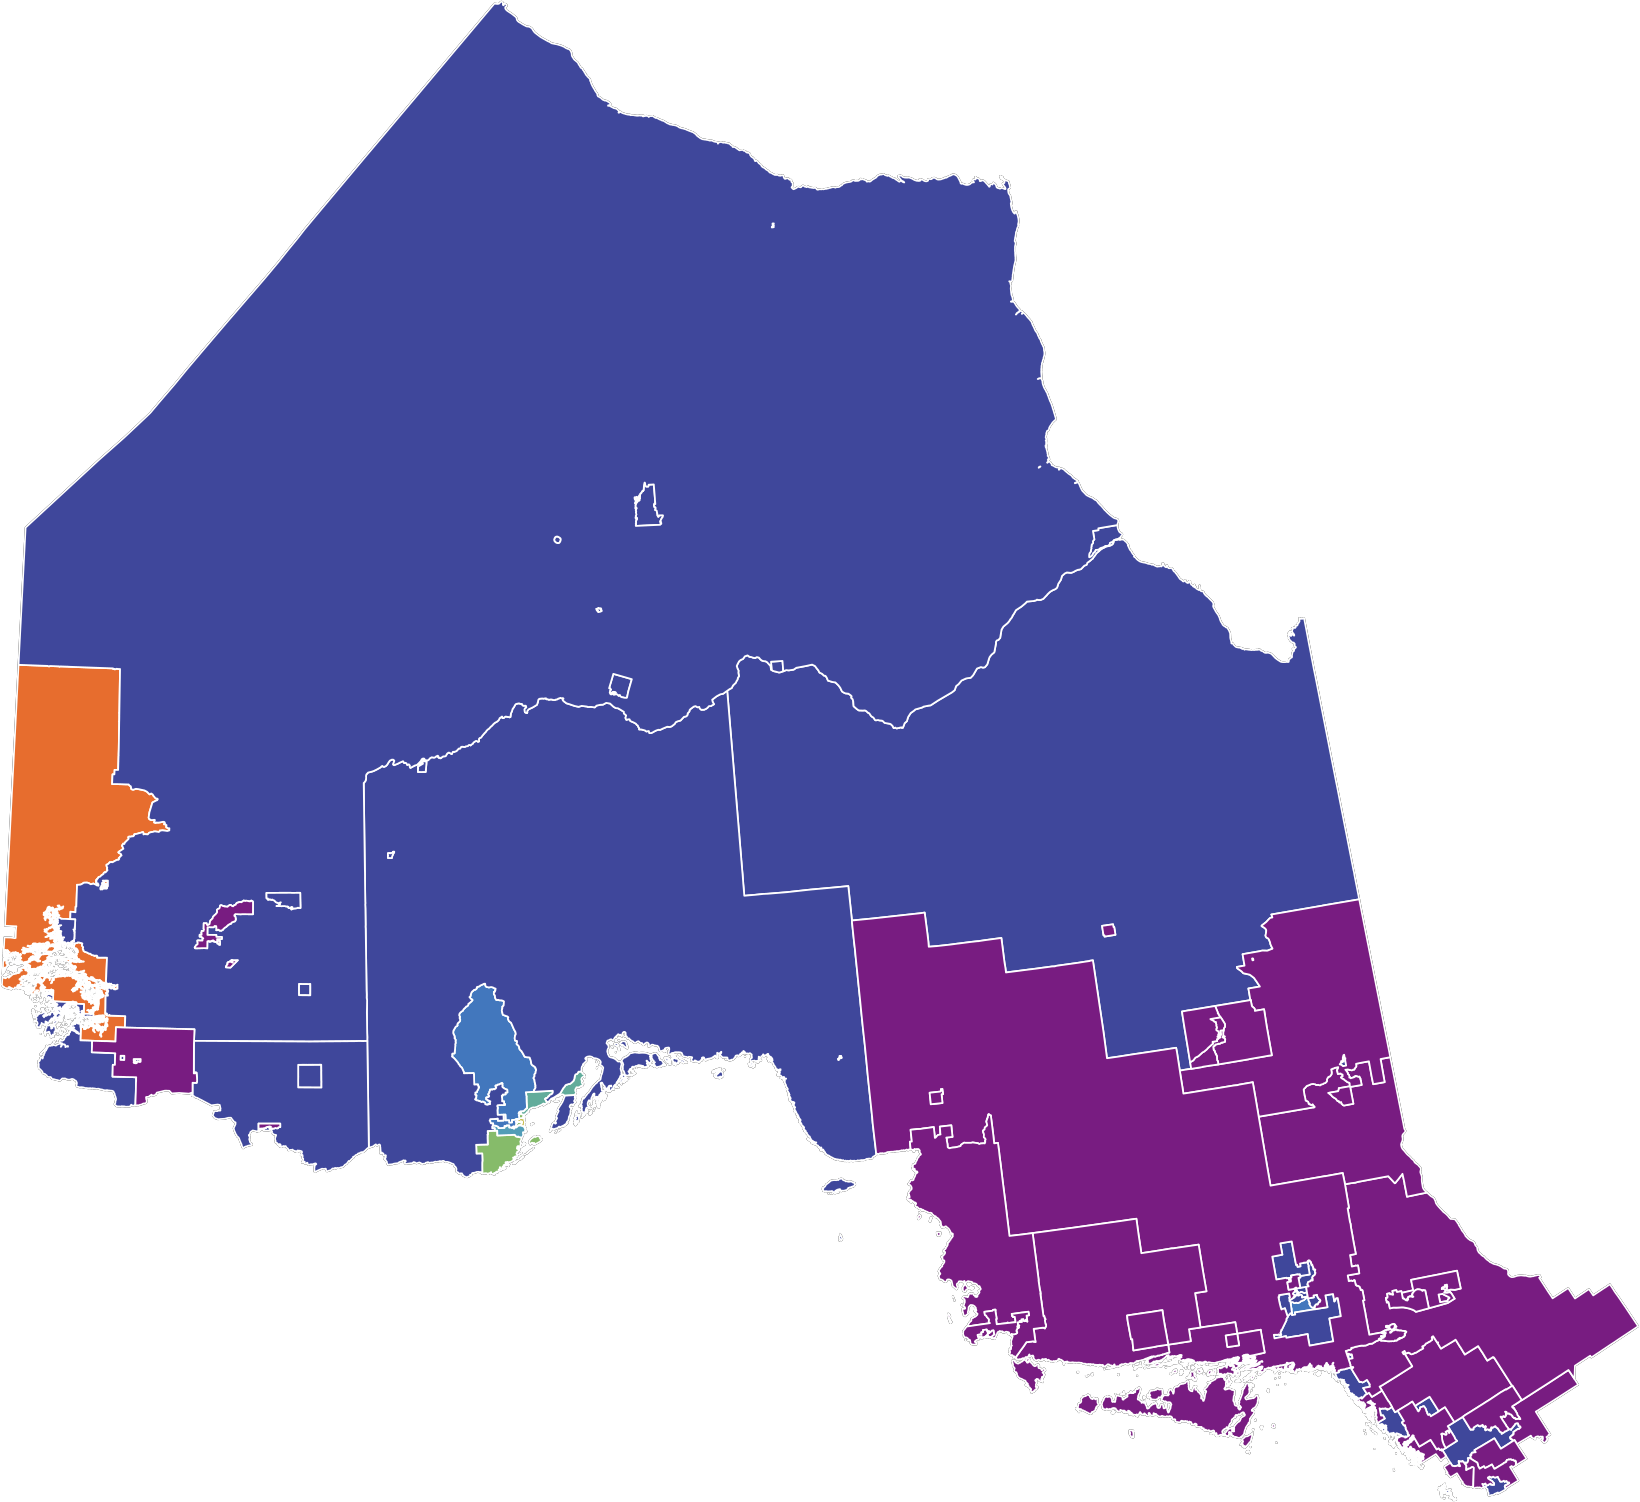
\includegraphics[width=.3\linewidth]{ontario-north.png} &
    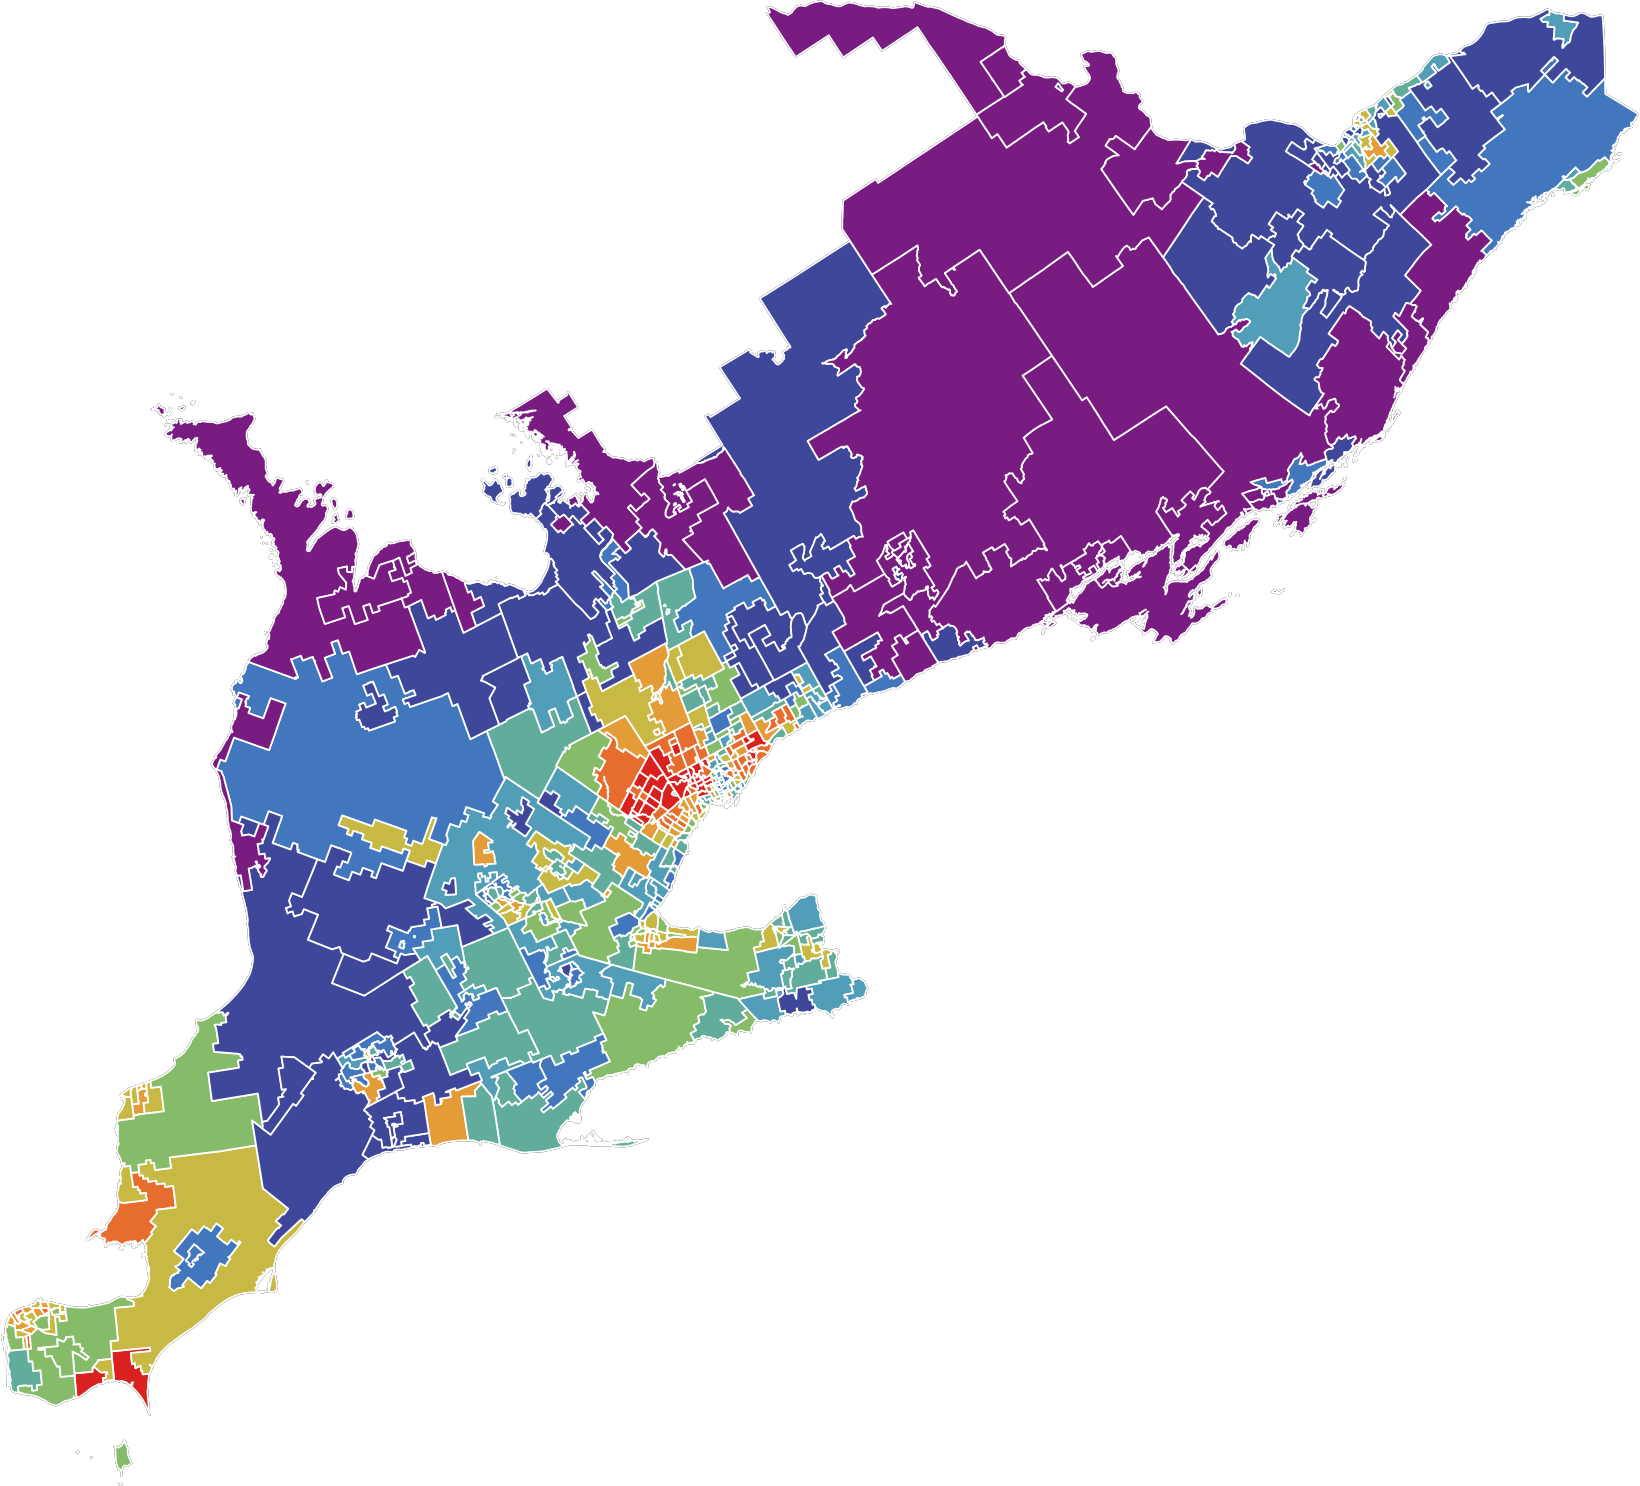
\includegraphics[width=.31\linewidth]{ontario-south.png} &
    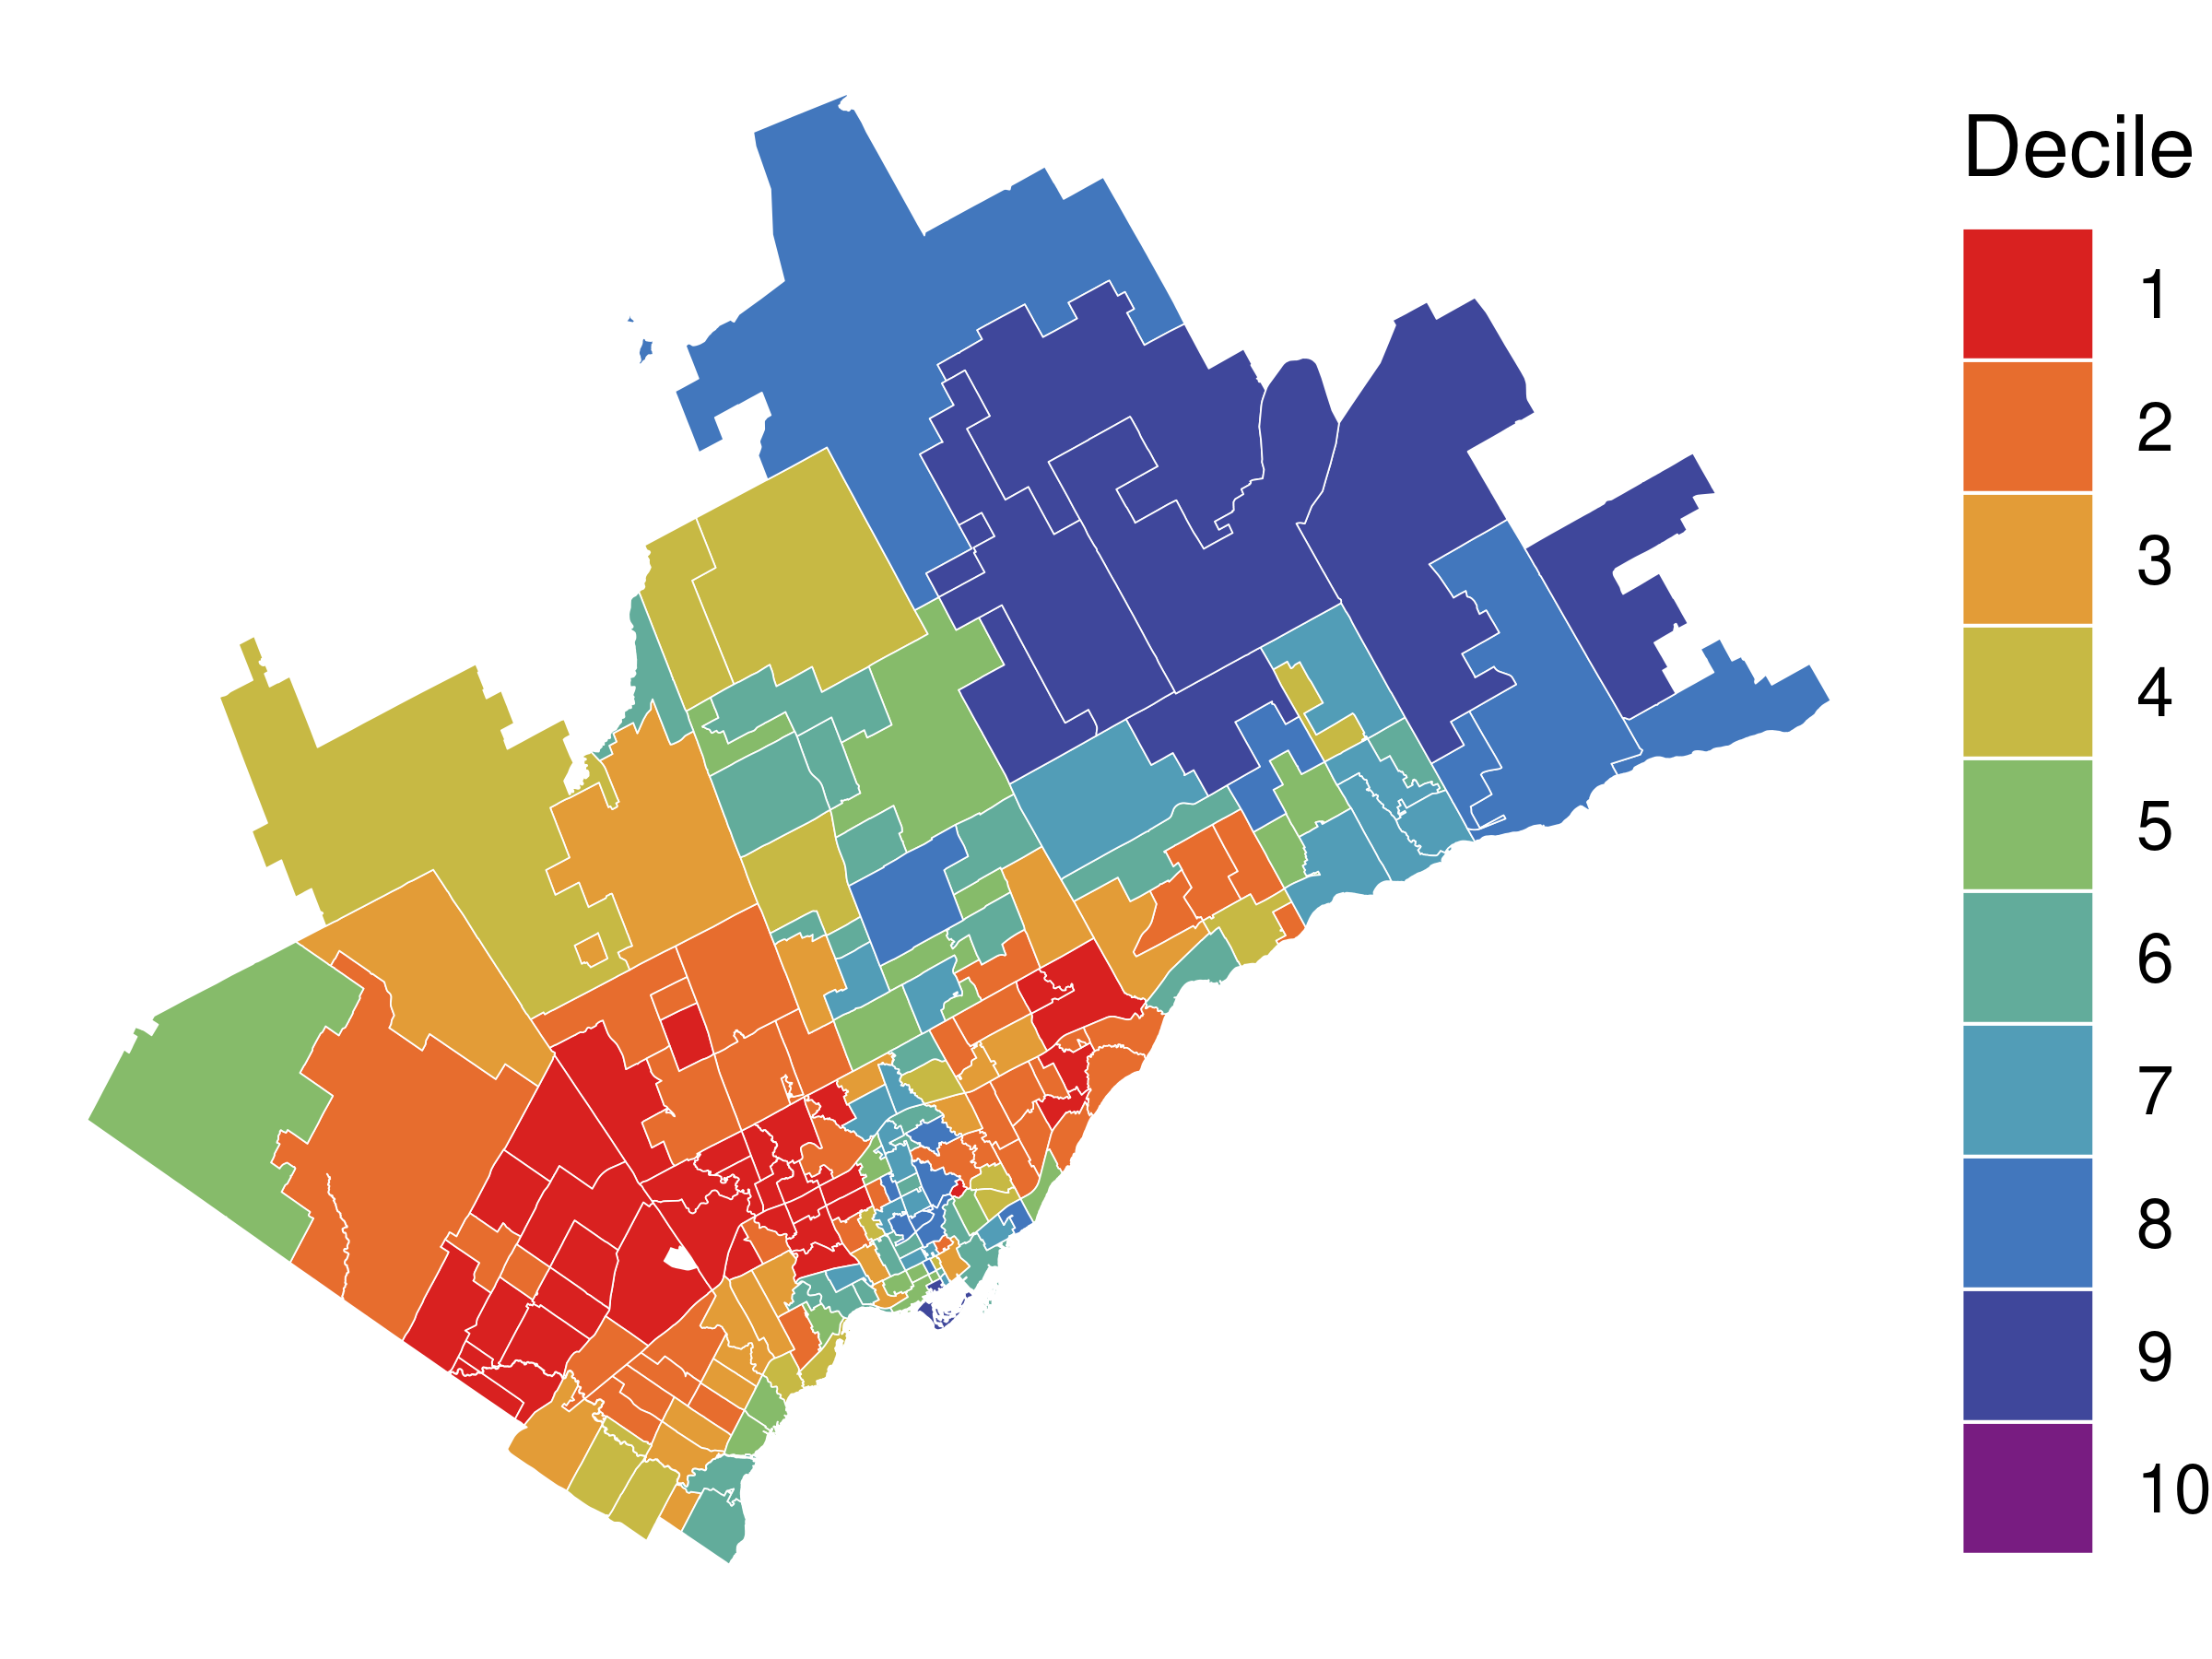
\includegraphics[width=.39\linewidth]{ontario-gta.png}
  \end{tabular}
  \caption{Ontario forward sorting areas (FSAs, $N=513$),
    stratified by decile rank in cumulative \covid cases between Dec 2020--May 2021;
    decile rank was used to group FSAs into 10 patches for transmission modelling.}
  \label{fig:map}
\end{figure}
% ==================================================================================================
\subsection{Data}\label{ex:data}
Ontario population sizes by age and FSA $P_{ga}$ were obtained from
the 2016 Canadian Census via Statistics Canada%
\footnote{\hreftt{https://www150.statcan.gc.ca/n1/en/catalogue/98-400-X2016008}}
and aggregated from 1-year age groups ($a_1$) into 5-year ($a_5$) and target ($a_*$) age groups as needed.
We obtained the final output contact matrices $C_{aa'y}$ from \cite{Prem2017},
for each of the ``home'', ``work'', ``school'', and ``others'' contact types,
as well as the population size of each 5-year age group used in \cite{Prem2017}.%
\footnote{\raggedright
  The rows for Canada in
  \texttt{contacts\_home.rdata},
  \texttt{contacts\_work.rdata},
  \texttt{contacts\_school.rdata}, and
  \texttt{contacts\_others.rdata}
  from \texttt{/generate\_synthetic\_matrices/output/syntheticcontactmatrices2020/} and
  \texttt{poptotal.rdata}
  from \texttt{/generate\_synthetic\_matrices/input/pop/}
  within \hreftt{https://github.com/kieshaprem/synthetic-contact-matrices/tree/67c824b}.}
We assumed that residence patch did not influence the numbers of contacts formed per person,
% MH: Wouldn't variability in population sizes per patch influence contacts per person?
% I thought we were incorporating variable age distribution?
although such a belief could easily be incorporated in the model,
perhaps in Eq.~(\ref{eq:X*.gagay}).
\par
The mobility matrix $B_{gg'}$ between patches was derived using
private data on geolocation service usage among a sample of approximately 2\% of mobile devices in Ontario;
Appendix~\ref{app.mob} details the specific methods and assumptions used.
To summarize:
Each device was assigned a home FSA ($n$) based on
the most common location during overnight hours for each calendar month.
Visits to other FSAs ($n'$) by each device were used to estimate
the proportion of devices in each FSA that are expected to travel to each other FSA each day, averaged monthly.
This proportion was adjusted for potential changes to the denominator associated with intention to travel.
We also assumed that individuals not in the dataset (approximately 98\%) had
0.9 the odds of being mobile versus the individuals in the dataset,
% MH: Might be helpful to add rationale for some of these assumptions
and that a proportion of individuals who were not observed to travel to any other FSA
were still mobile within their residence FSA.
% MH: This is the first we have discussed intra-FSA mobility
% and we only outline assumptions for unobserved individuals.
% What about intra-FSA mobility of observed individuals who didn't travel to other FSAs?
% What about intra-FSA mobility of individuals who did travel to other FSAs?
% Also, wouldn't most people be mobile within home FSA
% to run critical errands such as grocery shopping?
% Does this mean that we are assuming some individuals are not mobile whatsoever?
% Think more explanation is needed here.
% NOTE: After reading through manuscript, see we discuss intra-FSA mobility in section A.3.3.
% Would specifically reference the appendix here.
Then, the contribution of each FSA to overall mobility of the patch/decile (group of FSAs)
was aggregated as follows:
\begin{equation}\label{eq:Bgg}
  B_{gg'} = \sum_{n \in S_g}\sum_{n' \in S_g'} B_{nn'}
\end{equation}
where $S_g$ is the set of FSA $n$ corresponding to patch/decile $g$.
Mobility matrices were estimated for each month in the available dataset,
spanning Jan 2020--Jan 2021.
A reference period reflecting pre-pandemic conditions was defined as Jan--Feb 2020;
unless otherwise specified, all subsequent results use the average mobility patterns during that period
(Figure~\ref{fig:Bgg}).
We did not model any differences in mobility by age group,
although such differences could be included in the model by adding a relative rate in Eq.~(\ref{eq:P*}).
\begin{figure}
  \centering
  \begin{subfigure}{0.49\linewidth}
    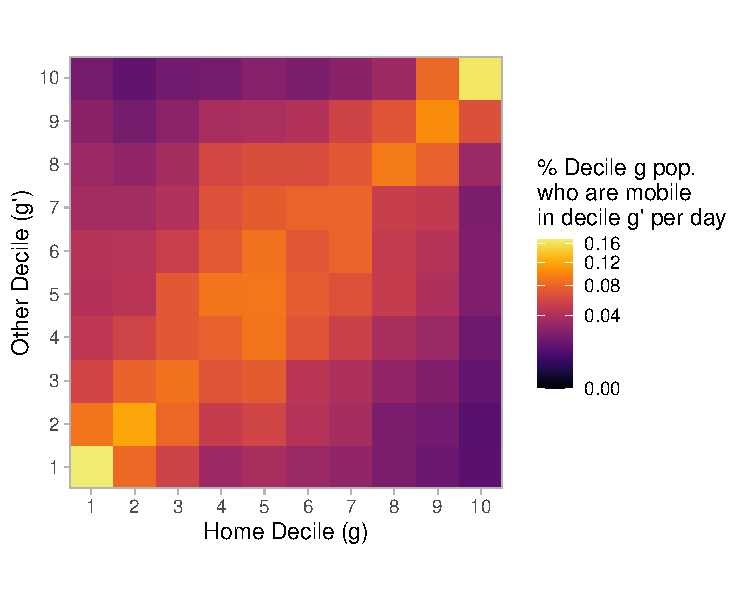
\includegraphics[width=\linewidth]{Bggi}
    \caption{Directly observed mobility: no data for mobility within the residence FSA}
    \label{fig:Bggo}
  \end{subfigure}\hfill%
  \begin{subfigure}{0.49\linewidth}
    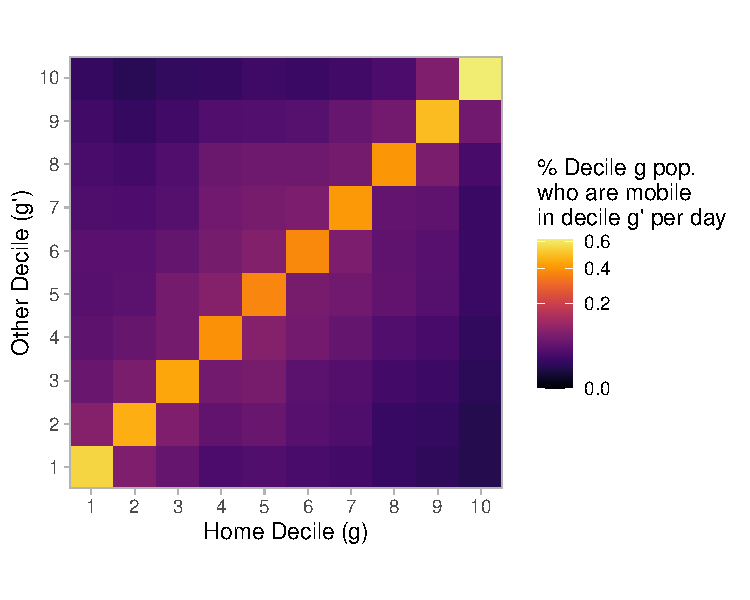
\includegraphics[width=\linewidth]{Bgg}
    \caption{Complete modelled mobility: including assumed mobility within the residence FSA}
    \label{fig:Bggd}
  \end{subfigure}
  \caption{Mobility matrix $B_{gg'}$, representing
    the proportion of individuals in decile (patch) $g$ who are expected to travel to decile $g'$ each day}
  \label{fig:Bgg}
  \floatfoot{Time period: Jan--Feb 2020 (average).
    Colour scales are square-root transformed to improve perception of smaller values.}
\end{figure}
\par
Finally, we specified the proportions of each contact type assumed to be formed with the home pool:
% MH: Why not state proportions that have been set for travel pool if we are stating for the home pool?
% Also may be helpful to add context here in how this connects to individual mobility.
% e.g. "we specified proprotions of each contact type assumed to be formed with the home pool
% (i.e. proportions of contact types for "not mobile" individuals).:
\begin{equation}
  h_y = \left\{
  \textsf{home}:   1,\enspace
  \textsf{work}:   0,\enspace
  \textsf{school}: 0,\enspace
  \textsf{others}: 0 \right\}
\end{equation}
The parameters $P_{ga}$, $C_{aa'y}$, $B_{gg'}$, and $h_y$ represent
the necessary inputs to our approach for calculating $C_{gag'a'y}$.
The following \S~\ref{ex:results} walks step-wise through the approach
and presents all major intermediate results.
\clearpage % TEMP
% ==================================================================================================
\subsection{Results}\label{ex:results}
Figure~\ref{fig:C4AAyi} illustrates the contact matrices $C_{aa'y}$ from \citet{Prem2017},
before and after the steps of unweighting by population age distributions, Eq.~(\ref{eq:C^u}),
and ensuring contact balancing, Eq.~(\ref{eq:C^ub}).
Figure~\ref{fig:C4AAyd} illustrates the differences in contact matrices between each step.
These differences can be explained as follows.
The Canadian age distribution used by \citet{Prem2017} (Figure~\ref{fig:Pga}, black dashed line),
is below the mean for the youngest and oldest age groups;
thus inverting the weighting by this age distribution
increases the contacts expected with these age groups (Figure~\ref{fig:C4AAyd01}).
By contrast, Figure~\ref{fig:C4AAyd12} is purely symmetric (and opposite about the central diagonal),
reflecting differences from the symmetric mean matrix.
\par
Figure~\ref{fig:C4**y} illustrates the unweighted and balanced contact matrices $C^{ub}_{aa'y}$
before and after bilinear interpolation and aggregation to the target age groups of interest, Eq.~(\ref{eq:Ca*}).
The final matrices $C^{ub}_{a_*a'_*y}$ include dominant horizontal streaks corresponding to larger age groups.
These streaks are expected, as more contacts are expected to form with larger ``other'' age groups.
Vertical streaks do not appear, as each column represents
the expected contacts for each person in the ``self'' age group,
not the total contacts formed by that age group.%
\footnote{The corresponding matrix of absolute contact $X_{aa'y} = C_{aa'y} P_{a'}$
  will be symmetric, and thus will include symmetric horizontal and vertical streaks.}
\begin{figure}
  \setlength{\abovecaptionskip}{.5\smallskipamount}
  \setlength{\belowcaptionskip}{.5\smallskipamount}
  \begin{subfigure}{\linewidth}
    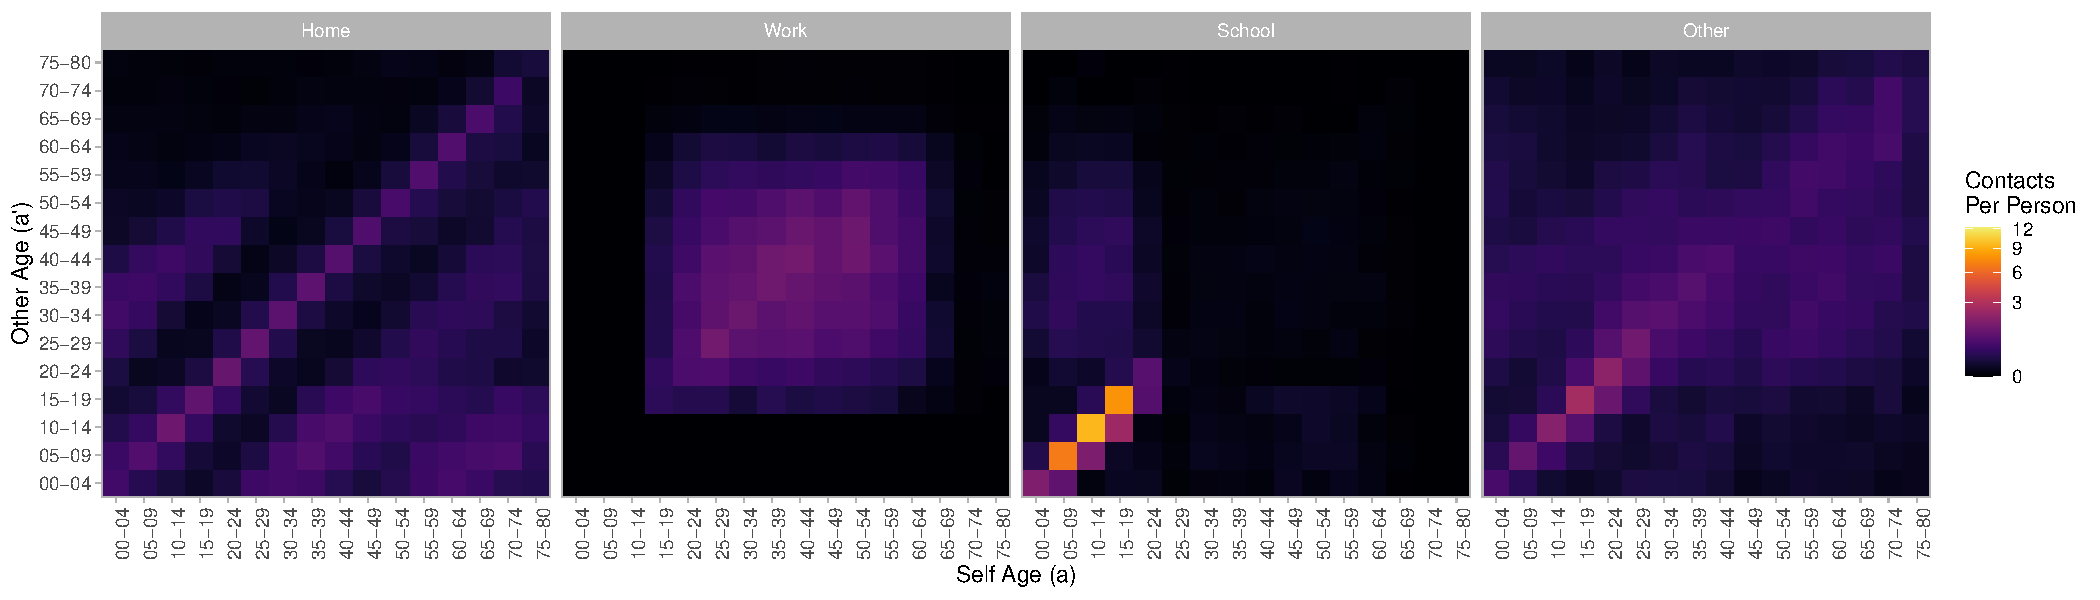
\includegraphics[width=\linewidth]{C4AAy0}
    \caption{Original contact matrix from \cite{Prem2017}, $C_{aa'y}$}
    \label{fig:C4AAy0}
  \end{subfigure}
  \begin{subfigure}{\linewidth}
    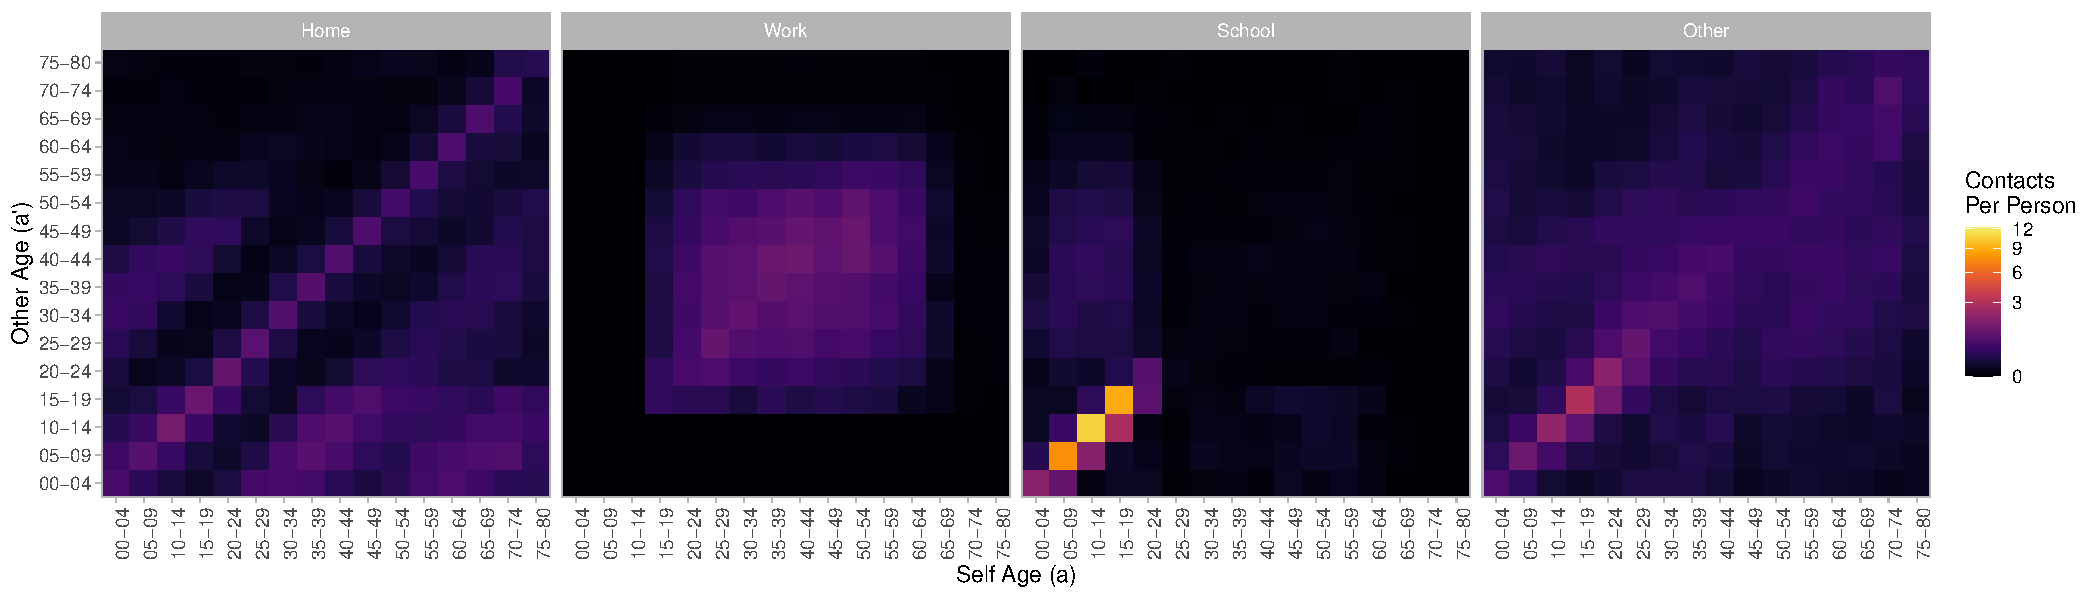
\includegraphics[width=\linewidth]{C4AAy1}
    \caption{Unweighted contact matrix, $C^u_{aa'y}$; result of Eq.~(\ref{eq:C^u})}
    \label{fig:C4AAy1}
  \end{subfigure}
  \begin{subfigure}{\linewidth}
    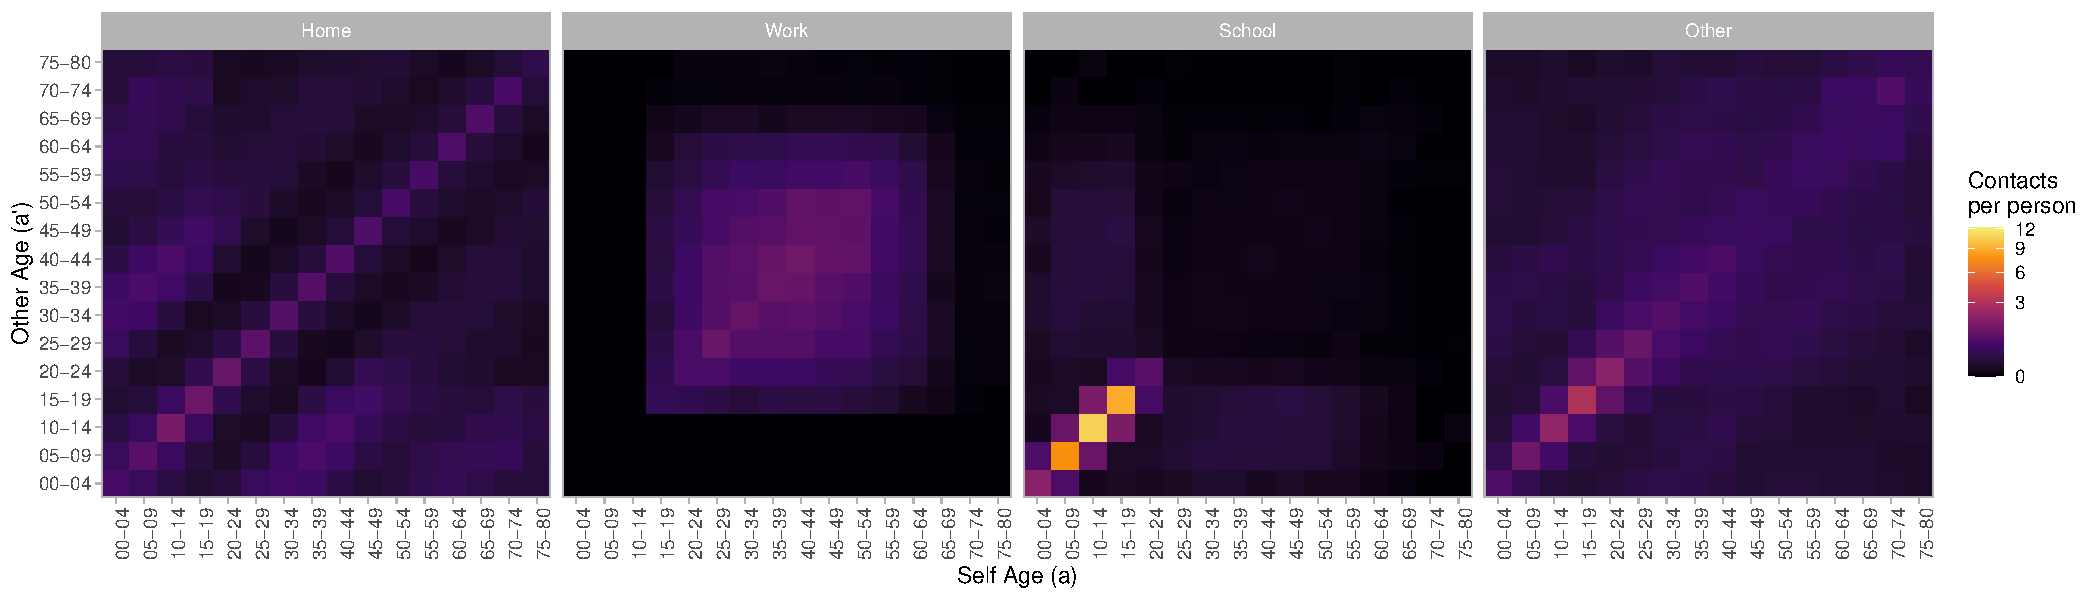
\includegraphics[width=\linewidth]{C4AAy}
    \caption{Balanced contact matrix, $C^{ub}_{aa'y}$; result of Eq.~(\ref{eq:C^ub})}
    \label{fig:C4AAy2}
  \end{subfigure}
  \caption{Intermediate results in obtaining unweighted and balanced age contact matrices $C^{ub}_{aa'y}$
    (expected number of type $y$ contacts per person per day in each age group $a$, with those other age groups $a'$)
    from population-weighted matrices $C_{aa'y}$ from \cite{Prem2017} which may not satisfy contact balancing}
  \label{fig:C4AAyi}
  \floatfoot{Colour scales are square-root transformed to improve perception of smaller values.}
\end{figure}
\begin{figure}
  \begin{subfigure}{\linewidth}
    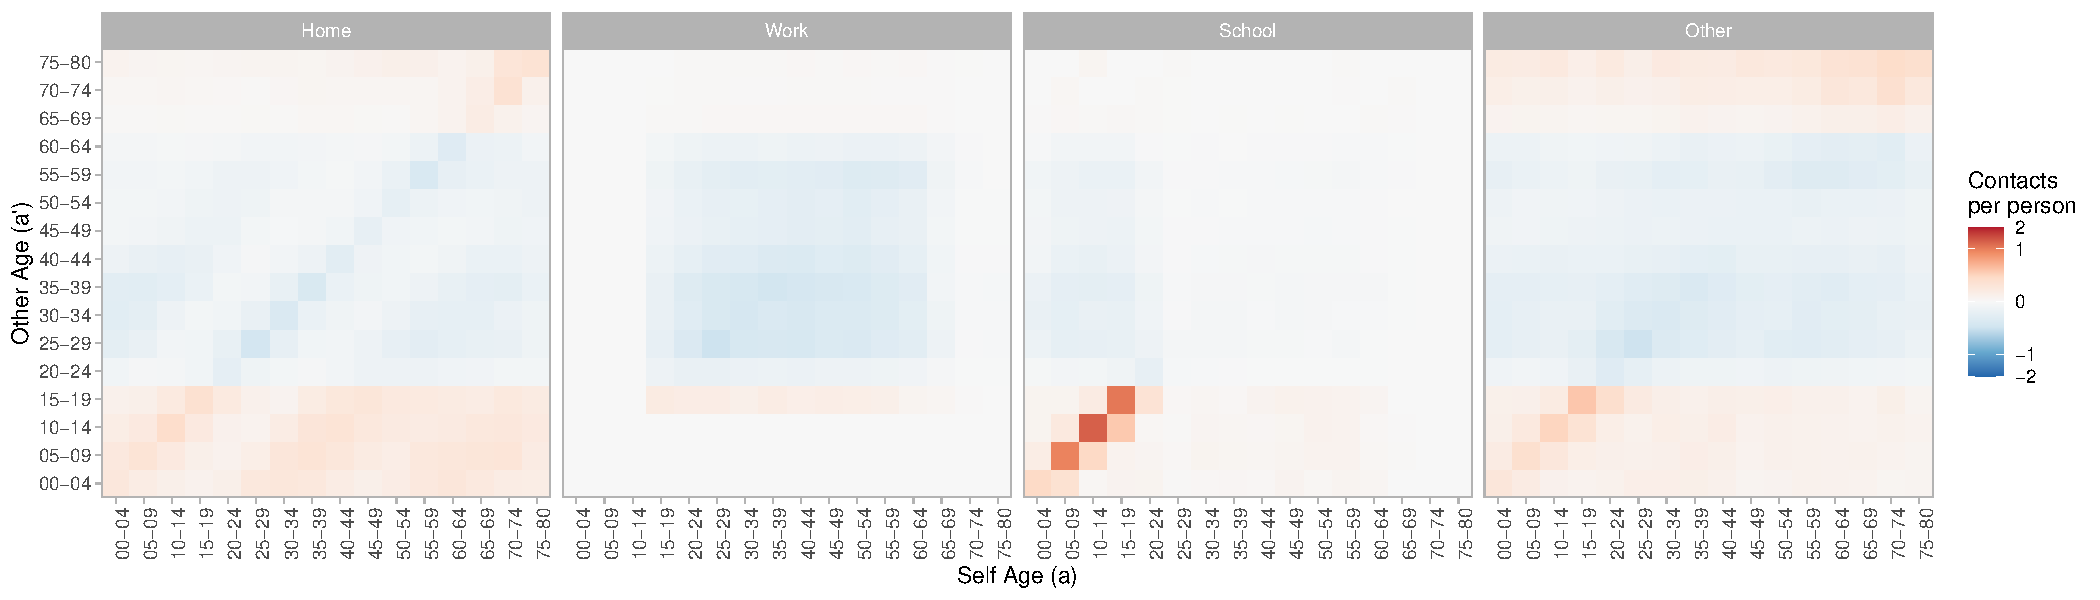
\includegraphics[width=\linewidth]{C4AAy-d01}
    \caption{Difference of Figure~\ref{fig:C4AAy1} and Figure~\ref{fig:C4AAy0}: $C^{u}_{aa'y} - C_{aa'y}$}
    \label{fig:C4AAyd01}
  \end{subfigure}
  \begin{subfigure}{\linewidth}
    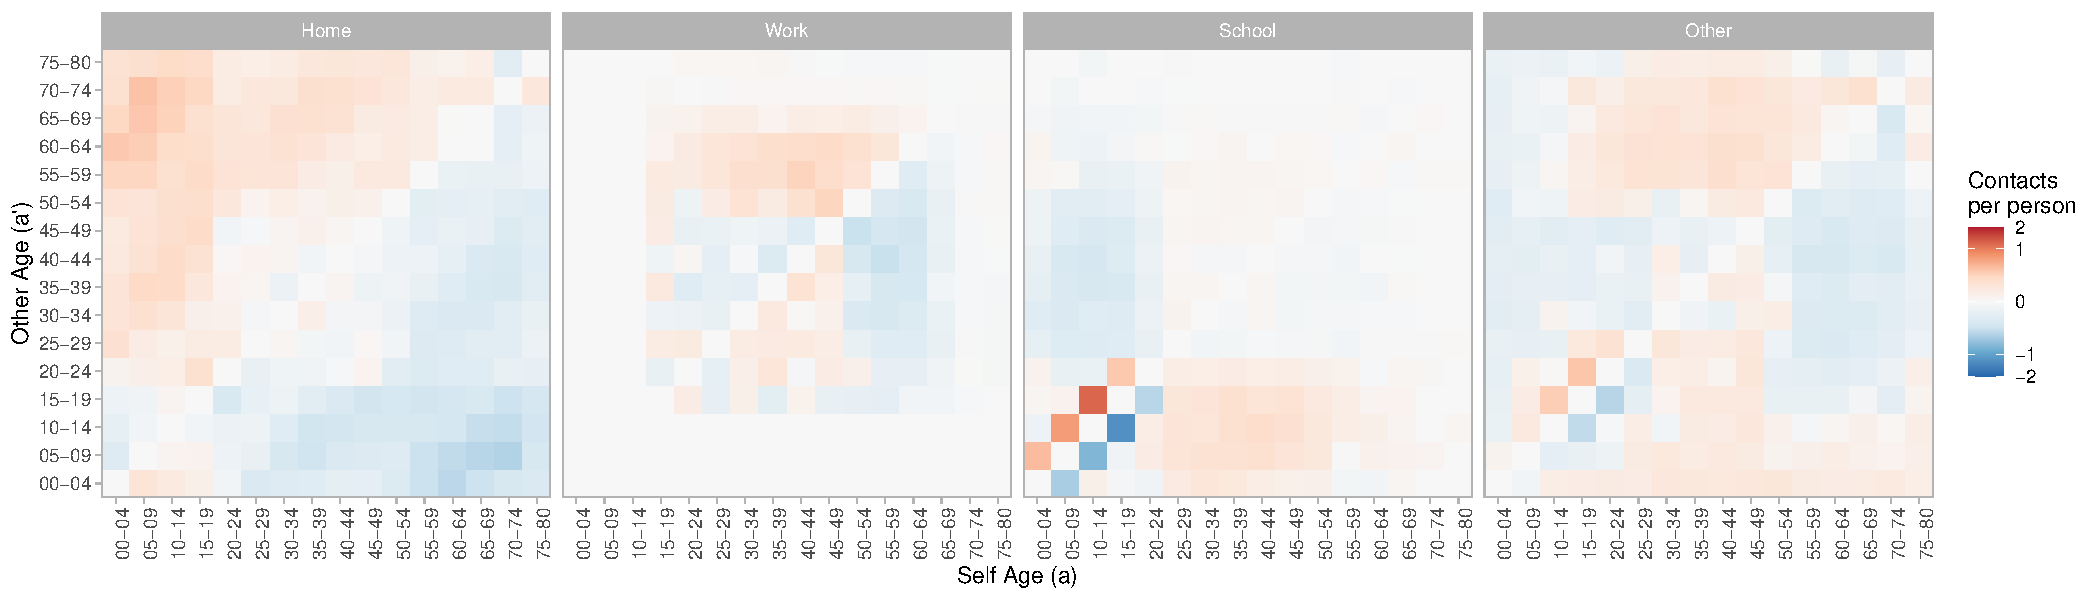
\includegraphics[width=\linewidth]{C4AAy-d12}
    \caption{Difference of Figure~\ref{fig:C4AAy2} and Figure~\ref{fig:C4AAy1}: $C^{ub}_{aa'y} - C^{u}_{aa'y}$}
    \label{fig:C4AAyd12}
  \end{subfigure}
  \begin{subfigure}{\linewidth}
    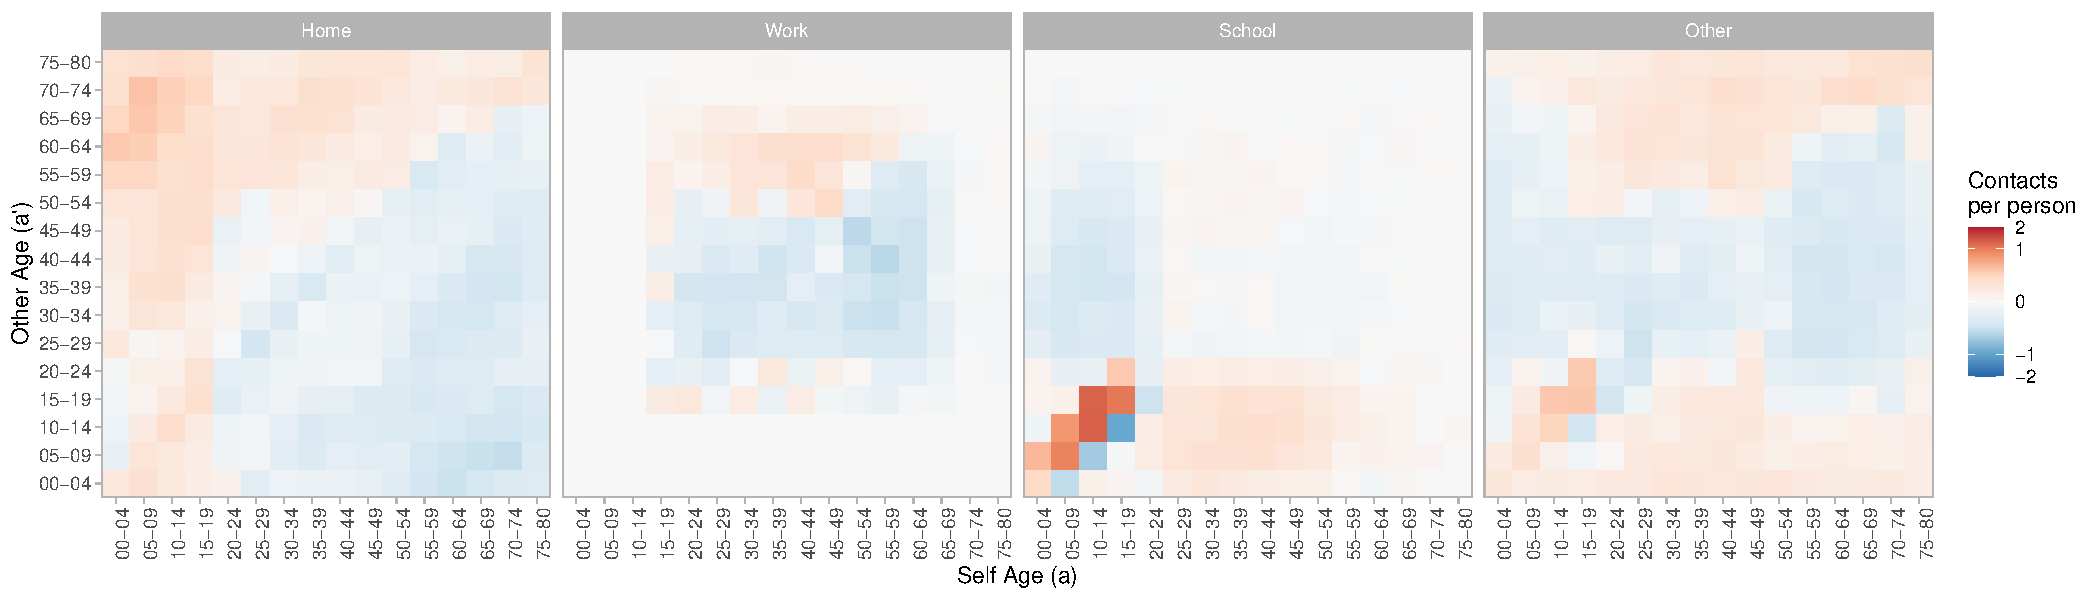
\includegraphics[width=\linewidth]{C4AAy-d02}
    \caption{Difference of Figure~\ref{fig:C4AAy2} and Figure~\ref{fig:C4AAy0}: $C^{ub}_{aa'y} - C_{aa'y}$}
    \label{fig:C4AAyd02}
  \end{subfigure}
  \caption{Differences between intermediate results shown in Figure~\ref{fig:C4AAyi}}
  \label{fig:C4AAyd}
\floatfoot{Colour scales are square-root transformed to improve perception of smaller values.}
\end{figure}
\begin{figure}
  \begin{subfigure}{\linewidth}
    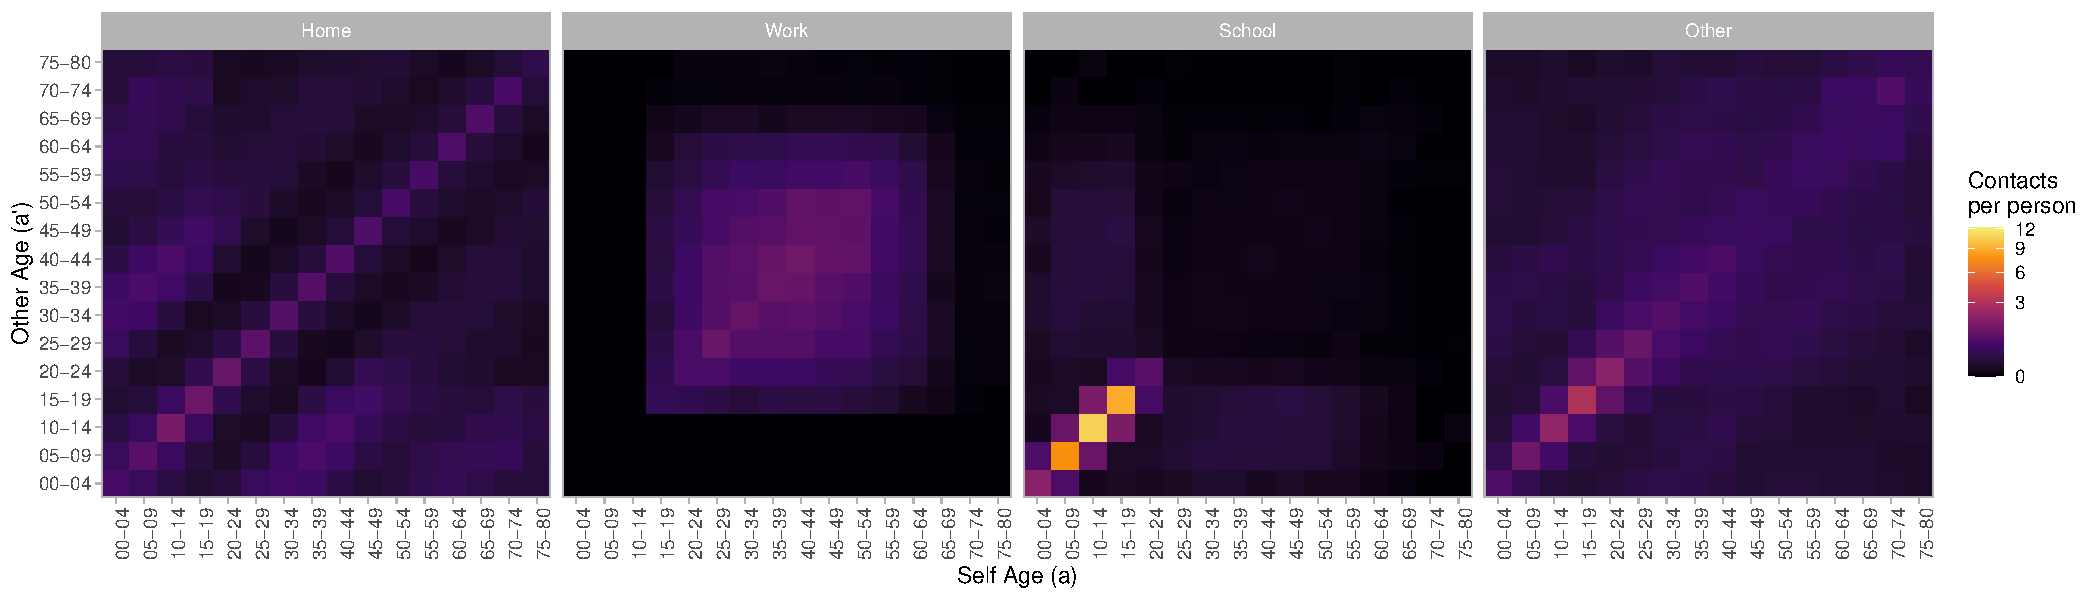
\includegraphics[width=\linewidth]{C4AAy}
    \caption{Original age groups $C^{ub}_{a_5a'_5y}$; result of Eq.~(\ref{eq:C^ub}); identical to Figure~\ref{fig:C4AAy2}}
    \label{fig:C4AAy}
  \end{subfigure}
  \begin{subfigure}{\linewidth}
    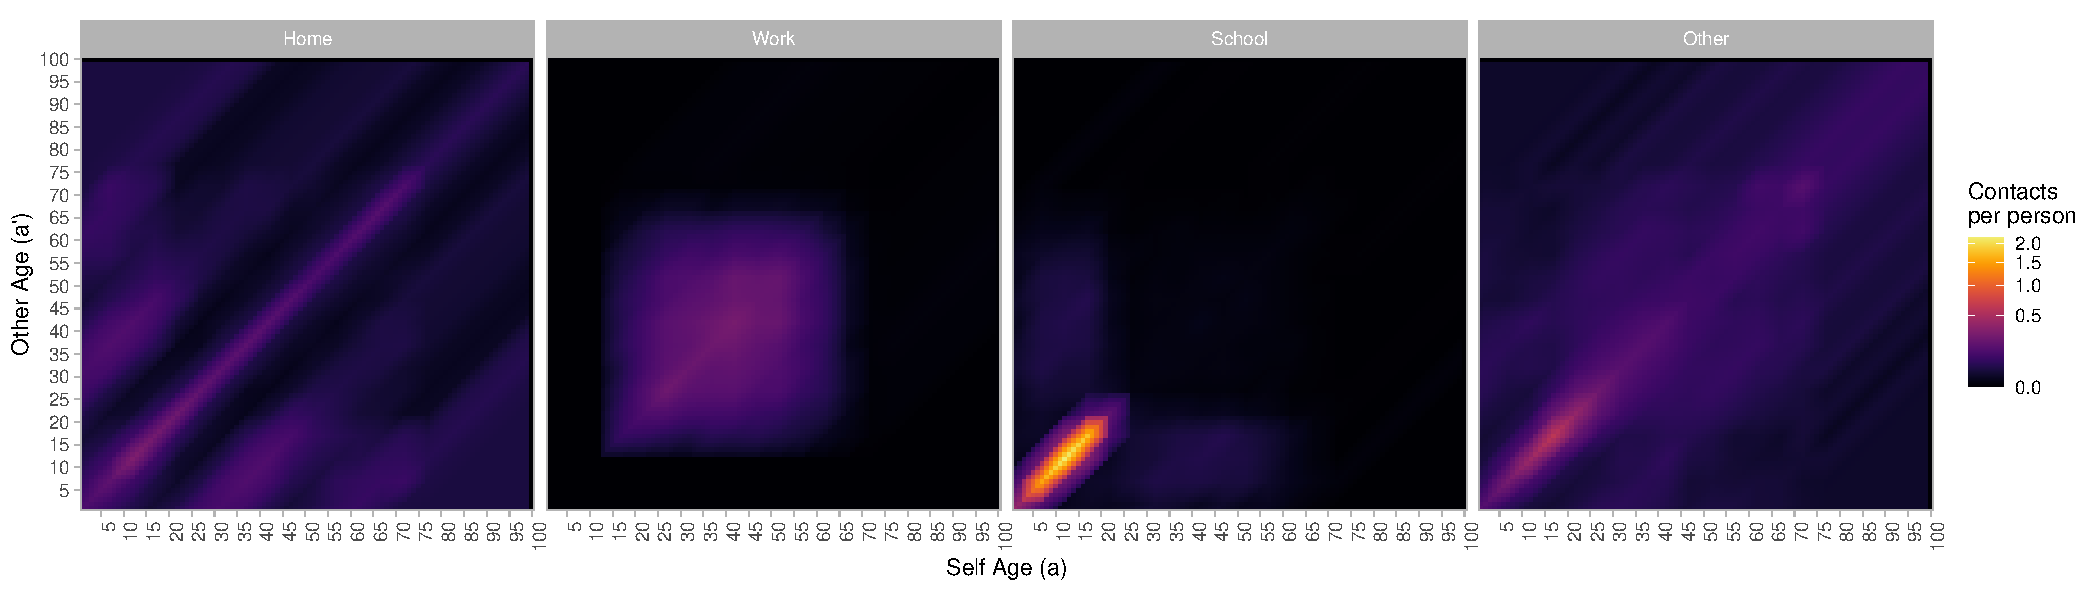
\includegraphics[width=\linewidth]{C411y}
    \caption{1-Year age groups $C^{ub}_{a_1a'_1y}$; result of diagonal edge padding and bilinear interpolation}
    \label{fig:C411y}
  \end{subfigure}
  \begin{subfigure}{\linewidth}
    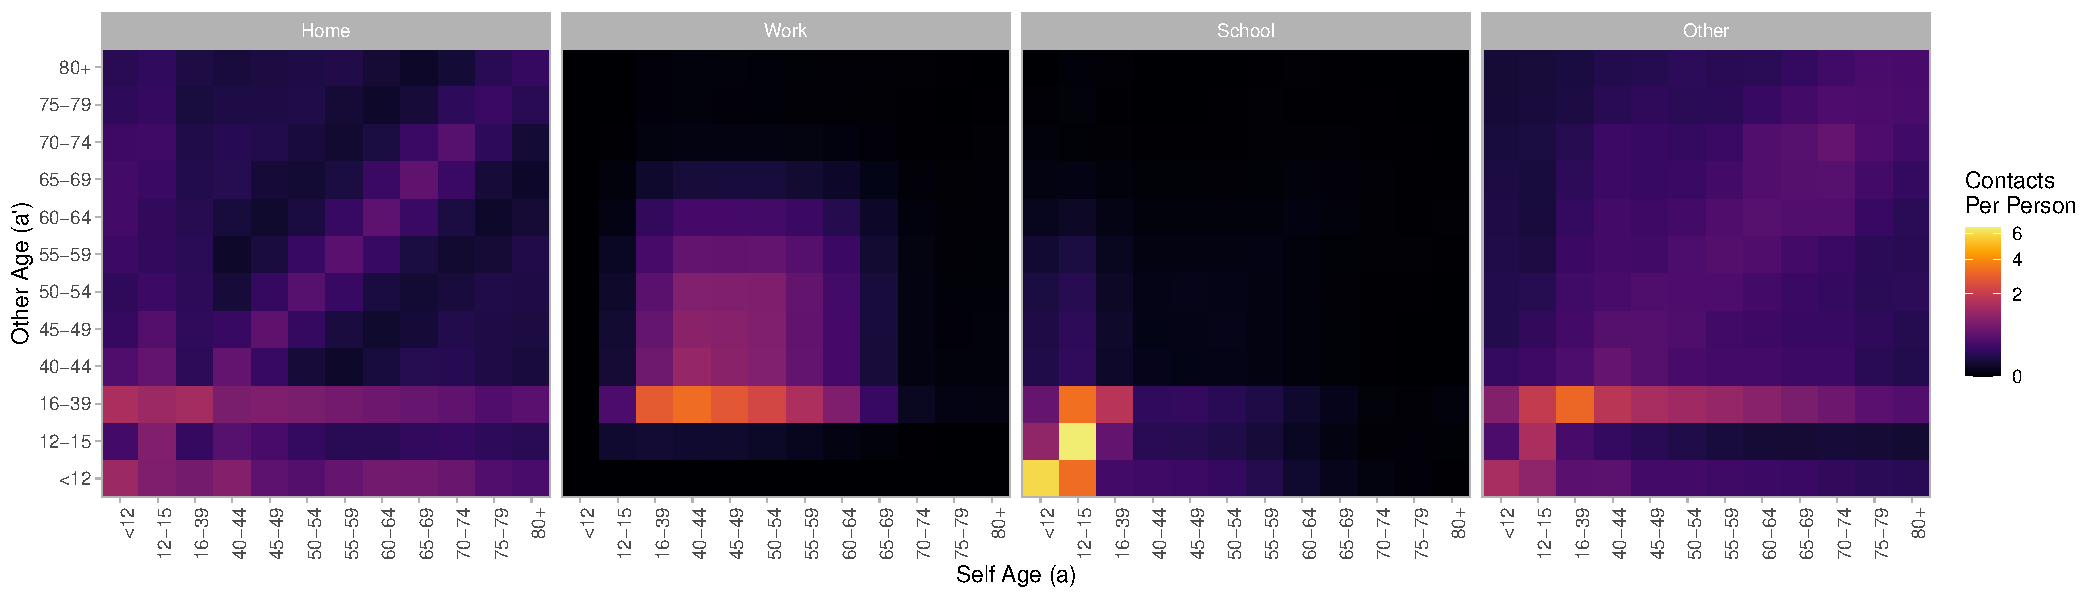
\includegraphics[width=\linewidth]{C4aay}
    \caption{Target age groups $C^{ub}_{a_*a'_*y}$; result of Eq.~(\ref{eq:Ca*})}
    \label{fig:C4aay}
  \end{subfigure}
  \caption{Intermediate results in obtaining age-restratified contact matrices $C^{ub}_{a_*a'_*y}$
    (expected number of type $y$ contacts per person per day in each age group $a_*$, with those from age groups $a'_*$)
    from matrices $C^{ub}_{a_5a'_5y}$ with 5-year age stratifications $a_5$}
  \label{fig:C4**y}
  \floatfoot{Colour scale is square-root transformed to improve perception of smaller values.
    The vertical streaks in (Figure~\ref{fig:C4aay}) corresponding to age groups 0--11 and 16--39 are expected,
    as more contacts will be formed with larger age groups.}
\end{figure}
\par
Figure~\ref{fig:C4Ay} plots the total expected contacts per person per day,
$C_{ay} = \sum_{a'} C_{aa'y}$, before and after each step.
% MH: Would clarify what step you are talking about
% given you havent referenced this since the first results paragraph.
Overall, patterns remained roughly consistent across transformations,
although some details among the large 16--39 age group are lost due to substantial averaging.
\begin{figure}
  \centering
  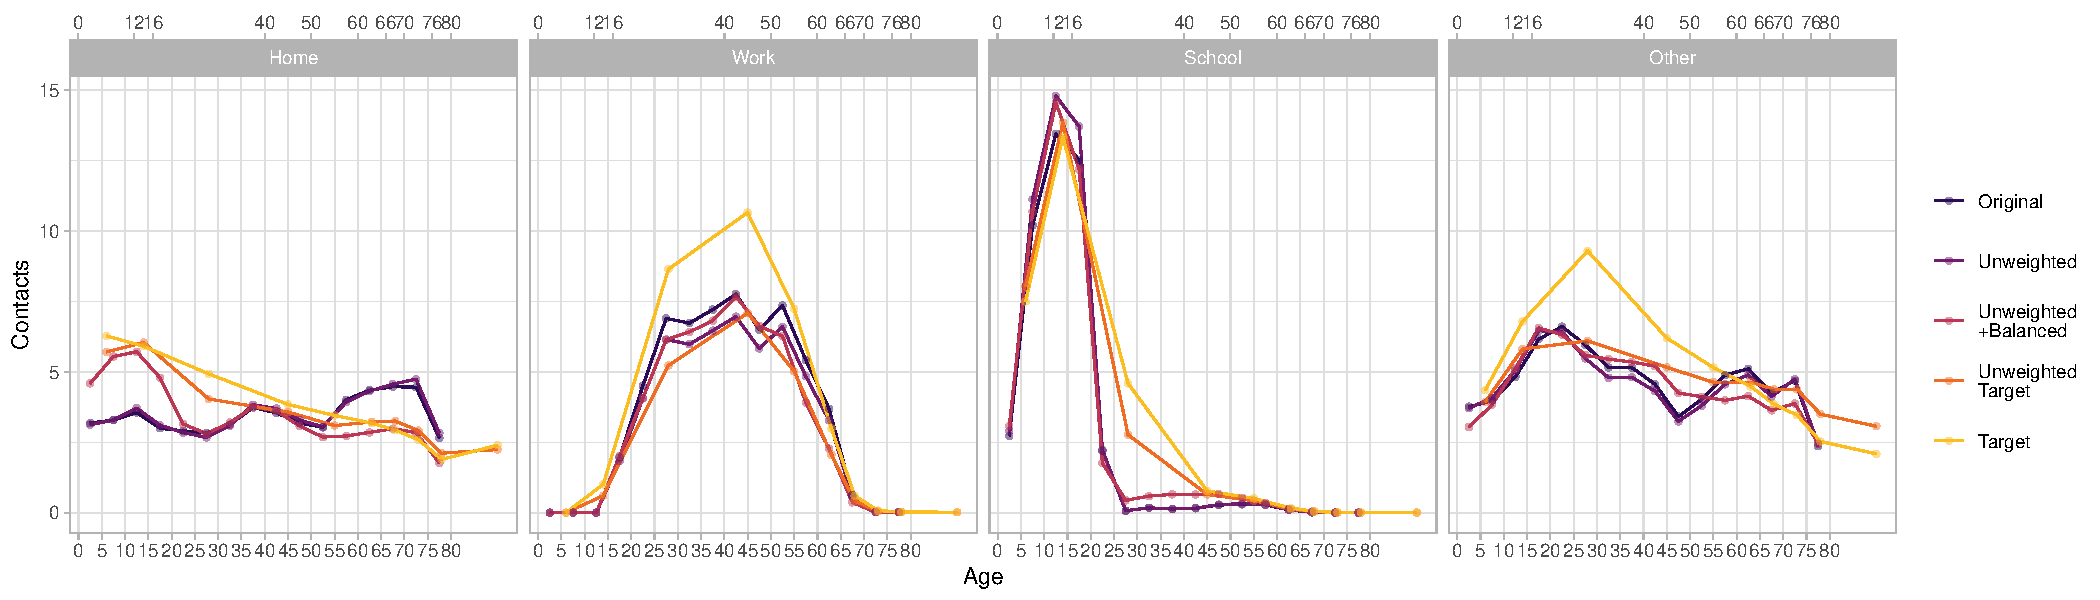
\includegraphics[width=\linewidth]{C4ay}
  \caption{Total contacts per person per day $C_{ay} = \sum_{a'} C_{aa'y}$
    for each intermediate step in obtaining $C^{ub}_{a_*a'_*y}$,
    stratified by contact type.}
  \label{fig:C4Ay}
  \floatfoot{Modelled contacts for each age group are plotted at the midpoint of the age group.
    The cut points for the original age groups $a_5$ from \cite{Prem2017} and
    the target age groups $a_*$ in our application
    are indicated on the bottom and top x-axis, respectively.}
\end{figure}
\par
Finally, Figure~\ref{fig:CX4y} illustrates the margins
(sum over ``other'' strata and population-weighted average over ``self'' strata)
of the complete mixing matrices $C_{gag'a'y}$, in terms of
age groups $a$~\&~$a'$ (Figure~\ref{fig:CX4aay}), and
patches/deciles $g$~\&~$g'$ (Figure~\ref{fig:CX4ggy}).
Such margins are computed as follows:
\begin{equation}\label{eq:Caay}
  C_{aa'y} = \left.\sum_{g} P_{ga} \sum_{g'} C_{gag'a'y} \middle/ \sum_{g} P_{ga} \right.
\end{equation}
\begin{equation}\label{eq:Cggy}
  C_{gg'y} = \left.\sum_{a} P_{ga} \sum_{a'} C_{gag'a'y} \middle/ \sum_{a} P_{ga} \right.
\end{equation}
The equivalent matrices for total number of contacts per person of all types
($C_{aa'}$ and $C_{gg'}$) are also given in Figures~\ref{fig:CXaay}~and~\ref{fig:CXggy}, respectively.
The marginal matrices $C_{aa'y}$ are identical to the input age mixing matrices from Eq.~(\ref{eq:Ca*}),
which could be used as an implementation check.
Since $h_y = 1$ for ``home'' contacts, $C_{gg'y}$ is an identity matrix.
The equivalent matrices for ``work'', ``school'', and ``others'' contact types
also feature a strong diagonal, due to a strong diagonal in the source mobility matrix $B_{gg'}$
(which includes assumptions about the mobility of some individuals within their own FSA).
However, the off-diagonal elements are less clustered towards the central diagonal
versus the mobility matrix $B_{gg'}$ (Figure~\ref{fig:Bgg});
mobile individuals from patches $g$ and $g'$ may form contacts
not only when either travels to the others' patch,
but also when they both travel to a third patch.
Thus, the connectivity of the network is greater than the mobility matrix alone would suggest,
but still less than random mixing.
% MH: Wording is a bit awkward here
\begin{figure}
  \begin{subfigure}{\linewidth}
    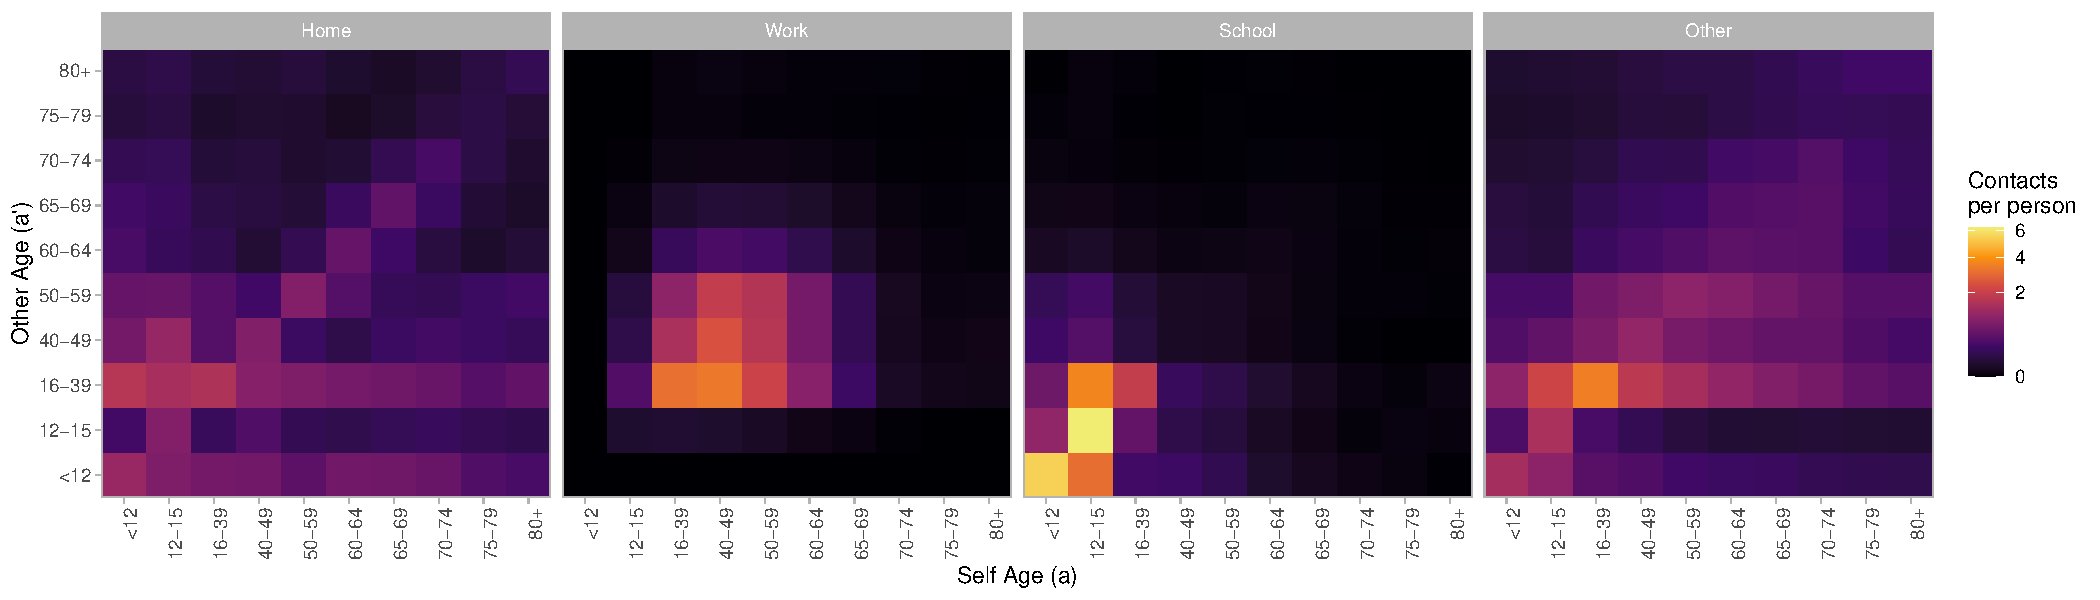
\includegraphics[width=\linewidth]{CX4aay}
    \caption{Stratified by age groups and contact type; from Eq.~(\ref{eq:Caay})}
    \label{fig:CX4aay}
  \end{subfigure}
  \begin{subfigure}{\linewidth}
    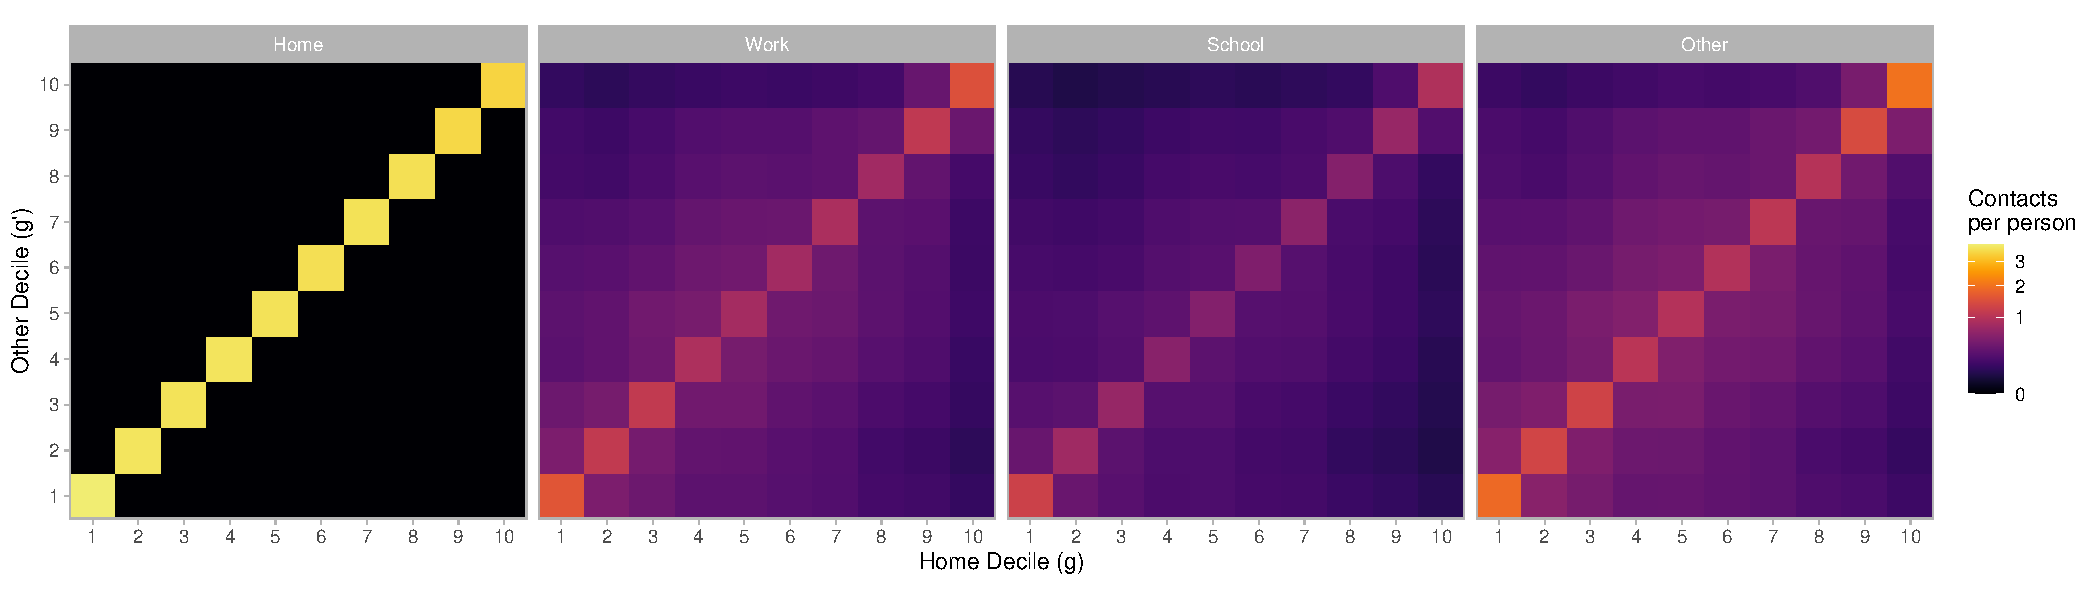
\includegraphics[width=\linewidth]{CX4ggy}
    \caption{Stratified by patches/deciles and contact type; from Eq.~(\ref{eq:Cggy})}
    \label{fig:CX4ggy}
  \end{subfigure}
  \begin{subfigure}{0.48\linewidth}
    \centering
    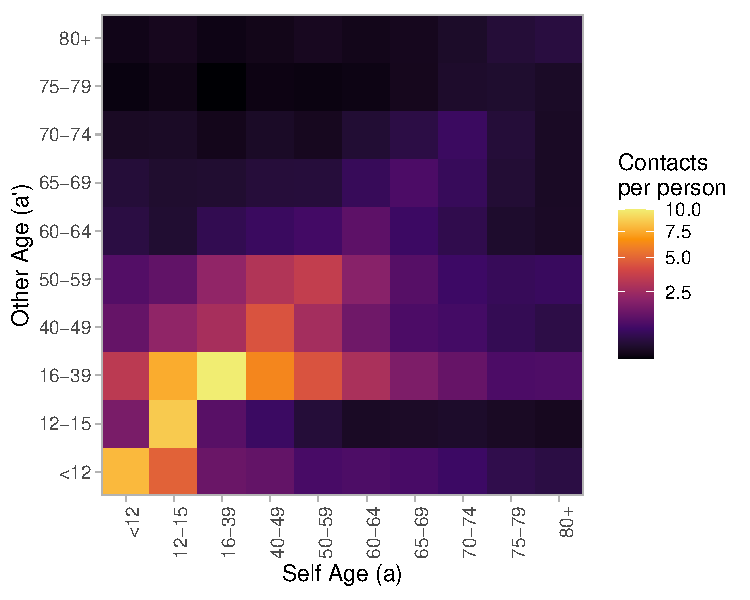
\includegraphics[width=\linewidth]{CXaay}
    \caption{Stratified by age groups (all types)}
    \label{fig:CXaay}
  \end{subfigure}\hfill%
  \begin{subfigure}{0.48\linewidth}
    \centering
    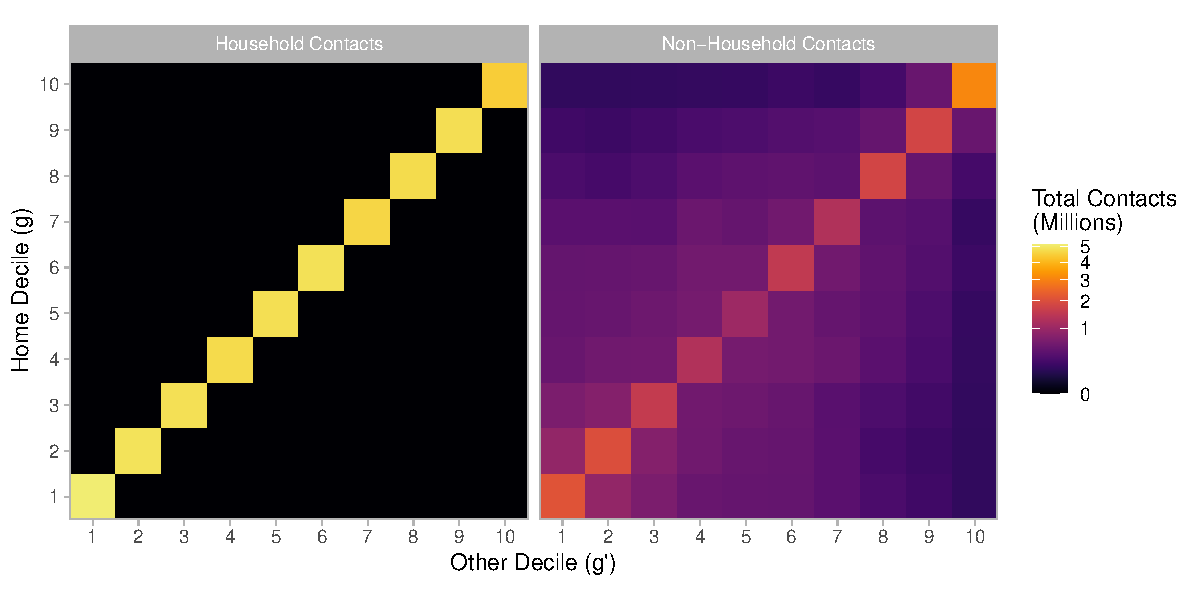
\includegraphics[width=\linewidth]{CXggy}
    \caption{Stratified by patches/deciles (all types)}
    \label{fig:CXggy}
  \end{subfigure}
  \caption{Expected contacts per person per day, stratified by age, patch/decile, and contact type,
    computed as the margins of the overall contact matrices $C_{gag'a'y}$}
  \label{fig:CX4y}
\end{figure}